\documentclass[12pt,a4paper]{article}

\usepackage[utf8]{inputenc}
\usepackage[T2A]{fontenc}
\usepackage[ukrainian]{babel}

\usepackage{geometry}
\geometry{left=2cm,right=2cm,top=2cm,bottom=2cm}

\usepackage{graphicx}
\usepackage{array,multirow}
\usepackage{booktabs}
\usepackage{caption}

\usepackage{enumitem}

\usepackage{amsmath}
\usepackage{xcolor}

\usepackage{minted}

\usemintedstyle{vs} % або monokai / vs / colorful
\setminted{linenos, breaklines, frame=single, fontsize=\small}

\usepackage{hyperref}

\begin{document}

    \begin{titlepage}

        % Картинка шапки (по центру, з відступом від верху)
        \begin{center}
\includegraphics[width=0.7\textwidth]{../../../../TITLES/letterhead.png}\end{center}

        \begin{center}
            \large Національний технічний університет України\\
            «Київський політехнічний інститут імені Ігоря Сікорського»\\[1em]
            Факультет інформатики та обчислювальної техніки\\
            Кафедра обчислювальної техніки
        \end{center}

        \vfill

        \begin{center}
            \textbf{\LARGE Вступ до операційної системи Linux. Курсова робота}\\[1.5em]
            \textbf{\Large Завдання №3}\\[1em]
            «Створення bash-скрипта за варіантом»
        \end{center}

        \vfill

        \begin{flushright}
            Виконав: студент 2 курсу ФІОТ, гр. ІО-41\\
            \textit{Давидчук А.~М.}\\[1em]
            Перевірив: \textit{Нікольський С.~С.}
        \end{flushright}

        \vfill

        \begin{center}Київ --- 2025\end{center}

    \end{titlepage}

    % Основний документ:

    \setlength{\parindent}{0em}

    \textbf{\underline{Тема:}} «Створення bash-скрипта за варіантом».
    
    \vspace{1em}

    \begin{center} \textbf{\Large Практична частина} \end{center}

    Опис всіх скриптів:

    \begin{enumerate}[label=\arabic*., start=0, itemsep=0.6em, leftmargin=*, align=left]

\item Скрипт приймає два числові параметри.
Якщо 1-й параметр більше 2-го -- вивести відповідне повідомлення, а
також список псевдонімів (alias) вашої системи.
Якщо 1-й параметр не більше 2-го -- вивести відповідне
повідомлення, а також розмір файлу скрипта (назва скрипта має
визначатися всередині самого скрипта).

\item В порядку зростання вивести на екран вагу та назву 3-х найбільш
“важких” директорій (просто файли пропускаються), що знаходиться
в директорії знаходження скрипта.

\item Пройтися по вмісту цільової директорії.
Для кожної директорії -- вивести повідомлення, що \emph{current\_dirname}
є директорією.
Якщо знайдений файл -- створити директорію \emph{current\_filename}\_dir,
і перемістити файл в неї. Вивести повідомлення, що
\emph{current\_filename} переміщений.

\item Згенерувати та записати до файлу 5 випадкових додатних чисел.
Вивести їх на екран. Видалити з файлу всі числа крім найменшого.
Результат вивести на екран.

\item Комбінація з двох маленьких скриптів.
Перший двічі рекурсивно проходить по вмісту цільової директорії,
спочатку видаляючи порожні файли, а потім порожні директорії.
Другий повинен запускати перший скрипт в новому вікні терміналу.
Створене вікно терміналу не повинно автоматично закриватися після
виконання скрипта.

\item Перенаправити результат виконання утиліти “top” в файл.
Обрізати кінець файлу, залишивши в ньому тільки перші n рядків. $n$
передаеться у якості параметру скрипта. Якщо параметр не було
задано, використовується значення 5.

\end{enumerate}

    Структура робочої директорії:

    \begin{minted}{text}
davydchuk@artem-laptop:~/Desktop/lab$ tree --charset=ascii
.
|-- 0file
|-- 1file
|   `-- file
|-- emptyfile.txt
|-- taskNo0.sh
|-- taskNo1.sh
|-- taskNo2.sh
|-- taskNo3.sh
|-- taskNo4_main.sh
|-- taskNo4_terminal.sh
`-- taskNo5.sh

3 directories, 9 files
    \end{minted}

    \newpage

    Код 1 скрипта (\texttt{taskNo0.sh}):

    \begin{minted}{bash}
#!/usr/bin/env bash
# taskNo0.sh - якщо $1 > $2 -> показати alias-и; інакше -> показати розмір цього скрипта
set -euo pipefail

[[ $# -eq 2 ]] || { echo "Використання: $0 <int1> <int2>"; exit 1; }
re='^-?[0-9]+$'
[[ $1 =~ $re && $2 =~ $re ]] || { echo "Параметри мають бути цілими числами"; exit 1; }

a=$1 b=$2
me=${BASH_SOURCE[0]}

if (( a > b )); then
  echo "Перший параметр ($a) > другого ($b). Alias-и:"
  alias 2>/dev/null || echo "(alias-и не визначені)"
else
  echo "Перший параметр ($a) <= другого ($b)."
  size=$(stat -c %s -- "$me" 2>/dev/null || wc -c < "$me")
  echo "Файл скрипта: $me"
  echo "Розмір скрипта: $size байт(и)"
fi
    \end{minted}

    Перевірка:
    \begin{minted}{bash}
davydchuk@artem-laptop:~/Desktop/lab$ ./taskNo0.sh
Використання: ./taskNo0.sh <int1> <int2>
davydchuk@artem-laptop:~/Desktop/lab$ ./taskNo0.sh 1 2
Перший параметр (1) <= другого (2).
Файл скрипта: ./taskNo0.sh
Розмір скрипта: 816 байт(и)
davydchuk@artem-laptop:~/Desktop/lab$ ./taskNo0.sh 2 1
Перший параметр (2) > другого (1). Alias-и:
    \end{minted}

    Код 2 скрипта (\texttt{taskNo1.sh}):

    \begin{minted}{bash}
#!/usr/bin/env bash
# taskNo1.sh - 3 найважчі піддиректорії біля скрипта; вивід за зростанням
set -euo pipefail

SCRIPT_DIR="$(cd -- "$(dirname -- "${BASH_SOURCE[0]}")" && pwd -P)"

# Якщо піддиректорій немає - повідомляємо і виходимо
if ! find "$SCRIPT_DIR" -mindepth 1 -maxdepth 1 -type d -print -quit | grep -q .; then
  echo "Поруч зі скриптом немає жодної піддиректорії"
  exit 0
fi

# Ланцюжок: перелік піддиректорій → їх розмір (у байтах) → топ-3 найбільші → відсортовано за зростанням
find "$SCRIPT_DIR" -mindepth 1 -maxdepth 1 -type d -print0 \
| xargs -0 -r du -sB1 \
| sort -n \
| tail -n 3 \
| sort -n \
| while read -r bytes path; do
    if command -v numfmt >/dev/null 2>&1; then
      human=$(numfmt --to=iec --suffix=B --format="%.1f" "$bytes")
    else
      human="${bytes}B"
    fi
    printf "%s\t%s\n" "$human" "${path##*/}"
  done
    \end{minted}

    Перевірка:
    \begin{minted}{bash}
davydchuk@artem-laptop:~/Desktop/lab$ ./taskNo1.sh
4,0KB 0file
8,0KB 1file
    \end{minted}

    Код 3 скрипта (\texttt{taskNo2.sh}):

    \begin{minted}{bash}
#!/usr/bin/env bash
# taskNo2.sh - пройтись по вмісту каталогу
set -euo pipefail

TARGET_DIR="${1:-.}"
[[ -d "$TARGET_DIR" ]] || { echo "Помилка: це не директорія: $TARGET_DIR" >&2; exit 1; }

# Перебір лише першого рівня (включно з прихованими). Отримаємо БАЗОВІ імена через %P.
while IFS= read -r -d '' name; do
  path="$TARGET_DIR/$name"

  if [[ -d "$path" ]]; then
    printf "%s є директорією\n" "$name"

  elif [[ -f "$path" || ( -L "$path" && ! -d "$path" ) ]]; then
    dest="$TARGET_DIR/${name}_dir"
    mkdir -p -- "$dest"

    target="$dest/$name"
    if [[ -e "$target" ]]; then
      i=1
      while [[ -e "$dest/${name}.dup${i}" ]]; do ((i++)); done
      target="$dest/${name}.dup${i}"
    fi

    mv -- "$path" "$target"
    printf "%s переміщений\n" "$name"

  else
    printf "%s пропущено (не файл і не директорія)\n" "$name"
  fi
done < <(find "$TARGET_DIR" -mindepth 1 -maxdepth 1 -printf '%P\0' | sort -z)
    \end{minted}

    Перевірка:
    \begin{minted}{bash}
davydchuk@artem-laptop:~/Desktop/lab$ ./taskNo2.sh
0file є директорією
1file є директорією
emptyfile.txt переміщений
taskNo0.sh переміщений
taskNo1.sh переміщений
taskNo2.sh переміщений
taskNo3.sh переміщений
taskNo4_main.sh переміщений
taskNo4_terminal.sh переміщений
taskNo5.sh переміщений
davydchuk@artem-laptop:~/Desktop/lab$ tree --charset=ascii
.
|-- 0file
|-- 1file
|   `-- file
|-- emptyfile.txt_dir
|   `-- emptyfile.txt
|-- taskNo0.sh_dir
|   `-- taskNo0.sh
|-- taskNo1.sh_dir
|   `-- taskNo1.sh
|-- taskNo2.sh_dir
|   `-- taskNo2.sh
|-- taskNo3.sh_dir
|   `-- taskNo3.sh
|-- taskNo4_main.sh_dir
|   `-- taskNo4_main.sh
|-- taskNo4_terminal.sh_dir
|   `-- taskNo4_terminal.sh
`-- taskNo5.sh_dir
    `-- taskNo5.sh

11 directories, 9 files
    \end{minted}

    І для подальшього демонстрування виконання скриптів, я переміщу всі файли назад (тобто дерево файлів повернеться у стан до виконання скрипту \texttt{taskNo2.sh}):

    \begin{minted}{bash}
davydchuk@artem-laptop:~/Desktop/lab$ tree --charset=ascii
.
|-- 0file
|-- 1file
|   `-- file
|-- emptyfile.txt
|-- taskNo0.sh
|-- taskNo1.sh
|-- taskNo2.sh
|-- taskNo3.sh
|-- taskNo4_main.sh
|-- taskNo4_terminal.sh
`-- taskNo5.sh

3 directories, 9 files
    \end{minted}

    Код 4 скрипта (\texttt{taskNo3.sh}):

    \begin{minted}{bash}
#!/usr/bin/env bash
# taskNo3.sh - згенерувати 5 додатних чисел, записати у файл, лишити мінімальне
set -euo pipefail

out="${1:-numbers.txt}"

# Згенерувати 5 чисел (1..1e6), показати й записати у файл
nums=$(for _ in {1..5}; do echo $(( (RANDOM<<15 | RANDOM) % 1000000 + 1 )); done)
printf "%s\n" $nums | tee "$out" >/dev/null

echo "Згенеровані числа:"
printf "%s " $nums; echo

# Знайти мінімум і перезаписати файл лише ним
min=$(printf "%s\n" $nums | sort -n | head -n1)
printf "%s\n" "$min" > "$out"

echo "Мінімальне число (залишено у файлі $out): $min"
echo "Вміст файлу після очистки:"
cat "$out"
    \end{minted}

    Перевірка:
    \begin{minted}{bash}
davydchuk@artem-laptop:~/Desktop/lab$ ./taskNo3.sh
Згенеровані числа:
999923 649956 433307 786355 839671 
Мінімальне число (залишено у файлі numbers.txt): 433307
Вміст файлу після очистки:
433307
davydchuk@artem-laptop:~/Desktop/lab$ tree --charset=ascii
.
|-- 0file
|-- 1file
|   `-- file
|-- emptyfile.txt
|-- numbers.txt
|-- taskNo0.sh
|-- taskNo1.sh
|-- taskNo2.sh
|-- taskNo3.sh
|-- taskNo4_main.sh
|-- taskNo4_terminal.sh
`-- taskNo5.sh

3 directories, 10 files
davydchuk@artem-laptop:~/Desktop/lab$ cat numbers.txt
433307
    \end{minted}

    Код 5 скрипта (обгортки) (\texttt{taskNo4\_terminal.sh}):

    \begin{minted}{bash}
#!/usr/bin/env bash
# taskNo4_terminal.sh - відкрити НОВЕ вікно терміналу, запустити taskNo4_main.sh і залишити вікно відкритим
set -euo pipefail

SELF_DIR="$(cd -- "$(dirname -- "${BASH_SOURCE[0]}")" && pwd -P)"
MAIN="$SELF_DIR/taskNo4_main.sh"

# 1) Визначаємо ціль: якщо не задано - беремо поточну директорію В МОМЕНТ ЗАПУСКУ і робимо її абсолютною
RAW_TARGET="${1:-$(pwd -P)}"
# realpath з фолбеком
if ! TARGET="$(realpath -- "$RAW_TARGET" 2>/dev/null)"; then
  TARGET="$RAW_TARGET"
fi

[[ -x "$MAIN" ]] || { echo "Помилка: зроби виконуваним $MAIN (chmod +x taskNo4_main.sh)" >&2; exit 1; }

# Якщо немає GUI - виконаємо в поточному терміналі з паузою
if [[ -z "${DISPLAY:-}" && -z "${WAYLAND_DISPLAY:-}" ]]; then
  bash --noprofile --norc "$MAIN" "$TARGET" || true
  read -r -p "Натисни Enter, щоб завершити..." _
  exit 0
fi

# Команда для нового вікна: просто викликаємо main з АБСОЛЮТНОЮ ціллю, потім пауза
inner=$(printf "%q " "$MAIN" "$TARGET")
inner+=$'; echo; echo "Завершено"; read -n1 -s -r -p "Натисни будь-яку клавішу, щоб закрити..."'

if command -v gnome-terminal >/dev/null 2>&1; then
  gnome-terminal -- bash --noprofile --norc -c "$inner"
elif command -v konsole >/dev/null 2>&1; then
  konsole --noclose -e bash --noprofile --norc -c "$inner"
elif command -v xfce4-terminal >/dev/null 2>&1; then
  xfce4-terminal --hold -e bash --noprofile --norc -c "$inner"
elif command -v kitty >/dev/null 2>&1; then
  kitty bash --noprofile --norc -c "$inner"
elif command -v alacritty >/dev/null 2>&1; then
  alacritty -e bash --noprofile --norc -c "$inner"
elif command -v xterm >/dev/null 2>&1; then
  xterm -hold -e bash --noprofile --norc -c "$inner"
else
  echo "Не знайдено відомого GUI-термінала. Встанови, напр.: sudo pacman -S xterm" >&2
  exit 1
fi
    \end{minted}

    Код 5 скрипта (основна логіка) (\texttt{taskNo4\_main.sh}):

    \begin{minted}{bash}
#!/usr/bin/env bash
# taskNo4_main.sh - спершу видаляє порожні файли, потім порожні директорії (рекурсивно)
set -euo pipefail

DIR="${1:-.}"
[[ -d $DIR ]] || { echo "Помилка: '$DIR' не існує або не є директорією" >&2; exit 1; }

printf "Цільова директорія: %s\n" "$DIR"
printf "Крок 1: Знаходимо порожні файли\n"
find -P "$DIR" -type f -empty -print -delete || true

printf "\nКрок 2: Знаходимо порожні директорії\n"
find -P "$DIR" -depth -type d -empty -print -delete || true

echo -e "\nГотово: видалені порожні директорії"
    \end{minted}

    Перевірка:

    \begin{figure}[h!]

        \renewcommand{\thefigure}{\arabic{figure}} % робимо "3.1", "3.2" і т.д.

        \centering
        % Підставляєте потрібний шлях та розмір зображення:
        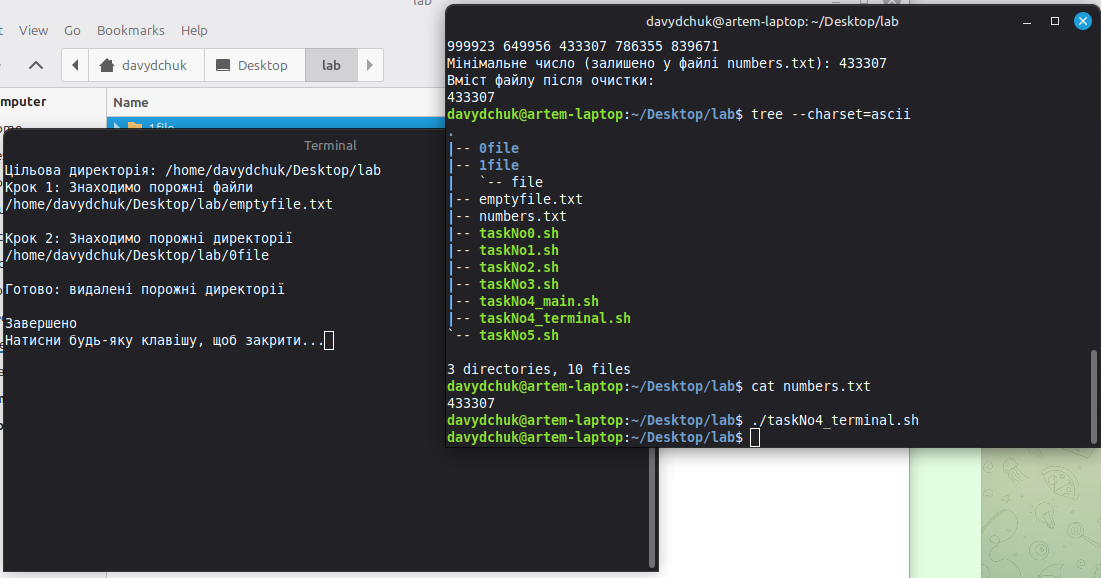
\includegraphics[width=1.0\textwidth]{task4.png}
        % Підпис (зазвичай під малюнком):
        \caption{Фото демонстрації відкриття нового вікна термінала}
        % Мітка для посилань у тексті (\ref{fig:...})
        \label{fig1:task4photo}

    \end{figure}

    \begin{minted}{bash}
davydchuk@artem-laptop:~/Desktop/lab$ tree --charset=ascii
.
|-- 1file
|   `-- file
|-- numbers.txt
|-- taskNo0.sh
|-- taskNo1.sh
|-- taskNo2.sh
|-- taskNo3.sh
|-- taskNo4_main.sh
|-- taskNo4_terminal.sh
`-- taskNo5.sh

2 directories, 9 files
    \end{minted}

    Звідси видно, що дійсно видалився файл \texttt{emptyfile.txt} і пуста директорія \texttt{0file}.

    \vspace{1em}

    Код 6 скрипта (\texttt{taskNo5.sh}):

    \begin{minted}{bash}
#!/usr/bin/env bash
# taskNo5.sh - записати в файл вивід top і залишити лише перші n рядків
set -euo pipefail

N="${1:-5}"
OUT="${2:-./top.txt}"

# Перевірка N: додатне ціле
[[ $N =~ ^[1-9][0-9]*$ ]] || { echo "Помилка: n має бути додатним цілим" >&2; exit 1; }

# 1) Повний знімок top
top -b -n1 > "$OUT"

# 2) Залишити лише перші N рядків (через тимчасовий файл - просто і прозоро)
tmp="$(mktemp "${OUT%.txt}.XXXXXX")"
head -n "$N" "$OUT" > "$tmp"
mv -f -- "$tmp" "$OUT"

echo "Записано у $OUT лише перші $N рядків виводу top"
    \end{minted}

    Перевірка:

    \begin{minted}{bash}
davydchuk@artem-laptop:~/Desktop/lab$ ./taskNo5.sh
Записано у ./top.txt лише перші 5 рядків виводу top
davydchuk@artem-laptop:~/Desktop/lab$ cat top.txt
top - 04:54:17 up  3:17,  1 user,  load average: 3,20, 1,51, 0,92
Tasks: 202 total,   1 running, 201 sleeping,   0 stopped,   0 zombie
%Cpu(s): 34,6 us, 19,2 sy,  0,0 ni, 46,2 id,  0,0 wa,  0,0 hi,  0,0 si,  0,0 st 
MiB Mem :   3915,9 total,    604,2 free,   2196,1 used,   1429,5 buff/cache     
MiB Swap:   2680,0 total,   2680,0 free,      0,0 used.   1719,7 avail Mem 
davydchuk@artem-laptop:~/Desktop/lab$ ./taskNo5.sh 15
Записано у ./top.txt лише перші 15 рядків виводу top
davydchuk@artem-laptop:~/Desktop/lab$ cat top.txt
top - 04:54:35 up  3:18,  1 user,  load average: 2,64, 1,49, 0,93
Tasks: 202 total,   3 running, 199 sleeping,   0 stopped,   0 zombie
%Cpu(s): 27,3 us, 18,2 sy,  0,0 ni, 54,5 id,  0,0 wa,  0,0 hi,  0,0 si,  0,0 st 
MiB Mem :   3915,9 total,    596,0 free,   2204,2 used,   1429,5 buff/cache     
MiB Swap:   2680,0 total,   2680,0 free,      0,0 used.   1711,6 avail Mem 

    PID USER      PR  NI    VIRT    RES    SHR S  %CPU  %MEM     TIME+ COMMAND
   1397 davydch+  20   0 4899492 324036 153548 R 158,3   8,1  54:05.86 cinnamon
   2192 davydch+  20   0   11,4g 599140 226544 S  33,3  14,9  18:46.10 firefox+
    897 root      20   0  525452 261032  83560 R  16,7   6,5   8:13.88 Xorg
   2403 davydch+  20   0   19,0g 397092 121416 S  16,7   9,9  17:55.97 Isolate+
      1 root      20   0   22408  13024   9184 S   0,0   0,3   0:01.79 systemd
      2 root      20   0       0      0      0 S   0,0   0,0   0:00.01 kthreadd
      3 root      20   0       0      0      0 S   0,0   0,0   0:00.00 pool_wo+
      4 root       0 -20       0      0      0 I   0,0   0,0   0:00.00 kworker+
    \end{minted}

    \textbf{\underline{Висновок:}} Реалізовано bash-скрипти для перевірки двох параметрів і
    виводу alias/розміру скрипта; визначення трьох найважчих директорій; проходження по вмісту теки з переміщенням файлів у
    \texttt{<name>\_dir}; генерації 5 випадкових чисел із залишенням мінімального; рекурсивного очищення порожніх файлів і
    тек та запуску в новому терміналі; знімка top з обрізанням до перших $n$ рядків;
    Демонстрація виводу результатів виконання цих скриптів підтвердила їх правильну реалізацію.

\end{document}